
\documentclass{article}

%========================================
\usepackage{tabularx, makecell, multirow }
\usepackage{syntonly}
%hpyerlien
\usepackage{hyperref}
%utf8
\usepackage[utf8]{inputenc}
%to solve footnote too high 
%(this helps fix footnote to bottom of the page)
\usepackage[bottom]{footmisc}
%array: aimed at tabular
\usepackage{array}
% sanxianbiao
\usepackage{booktabs}
% graphics
\usepackage{graphicx}
%math
\usepackage{amsmath}
%========================================

%----------------- new commands ----------
%            -{}-
\newcommand{\ac}[1]{\left\{ #1 \right\}}

\title{\textbf{IFT2105 Devoir1}}
\author{
    Samy Rasmy 20214818 \and Yuchen Hui 20150470}
\date{\today}


\begin{document}
\maketitle
\newpage
\section{Programme RÉPÉTER et TANQUE}

%%%%%%%% Question 1.a
\paragraph{a. Sommaire d'entiers}~{}\\

\begin{verbatim}
    #SOMME D'ENTIERS

    repeter r2 fois {
        inc(r5)
        r3    <-    PREMIERK(r5)
        r1 = DIV(r1, r3)
        repeter r1 fois{
            inc(r4)
        }
    }

    r0    <-    r4
\end{verbatim}

%%%%%%%% Question 1.b
\paragraph{b. FRACTRAN}~{}\\
\begin{verbatim}
    #FRACTRAN:
    #ON ASSUME QUE LES TABLEAUX SONT INDEXES A PARTIR DE 1 POUR TABLVAL

    tant que r5 != r3{
        inc(r5)
        r6    <-     TABLVAL(r1, x)
        r7     <-     TABLVAL(r2, x)
        r8    <-    PGCD(r6, r7)
        r6     <-     DIV(r6, r8)
        r7    <-    DIV(r7, r8)
        si EQ(MOD(MULT(r6, r4), r7), 0) {
            r3    <-    DIV(MULT(r4, r6), r7)
            r5    <-    0
        }
    }

    r0    <-    r4
\end{verbatim}
\newpage
\section{Langage régulier}

%%%%%%%% Question 2.a
\paragraph{a.}~$\Sigma = \{a,b\} \text{ et } L = \{w \in \Sigma^{*} | |w|_{a } = 2 \text{ ou } |w|_{b} = 3\}$ \\ 

\textbf{description textuelle:}
\begin{align}
     &M = \ac{Q,\Sigma, \delta, q_0, F}\nonumber\\
     &\text{où}\nonumber\\
     & Q = \ac{<a_ib_j> | i = 0,1,2,3; j = 0,1,2,3,4;}\nonumber\\
     &  q_0 = <a_0b_0>\nonumber\\
     &   F = \ac{<a_ib_j> | i = 2 or j = 3}\nonumber\\
     &   \delta \text{ est donné par}\nonumber\\
     &   \delta (<a_ib_j>,a) =<a_{i+1}b_j>, i = 0,1,2; \forall j; \nonumber\\
     &   \delta (<a_ib_j>,b) =<a_{i}b_{j+1}>, j = 0,1,2,3; \forall i; \nonumber\\
     &   \delta (<a_ib_j>,b) =<a_{i}b_{j}>, i = 3; \forall j; \nonumber\\
     &   \delta (<a_ib_j>,b) =<a_{i}b_{j}>, j = 4; \forall i;\nonumber 
\end{align}
\marginpar[]{\footnotesize{Bleu: État initial Vert: État acceptant}}
   
        
    %%picture
\begin{figure}[h]
    \centering
    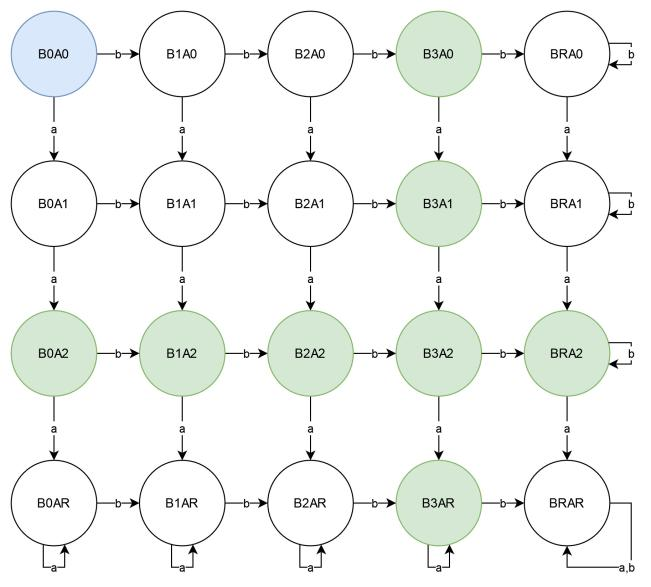
\includegraphics[scale = 0.45]{2a.jpg}
    \caption{solution 2.a}
    \label{fig.2a}
\end{figure}
\newpage

\paragraph{b.}~$\Sigma = \{a,b\} \text{ et } L = \{w \in \Sigma^{*} | |w|_{a } \equiv |w|_{b} +1 (\bmod 3)\}$ \\ 

\marginpar[]{\footnotesize{Bleu: État initial Vert: État acceptant}}
\begin{figure}[h]
    \centering
    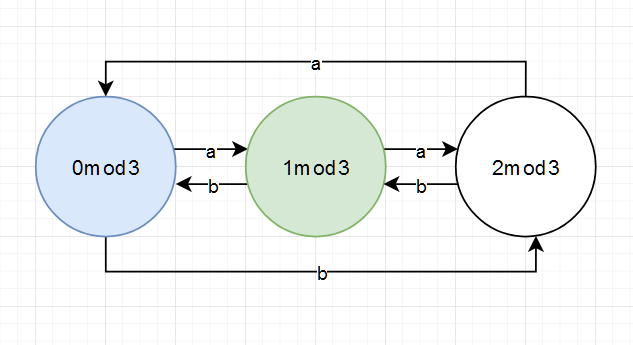
\includegraphics[scale = 0.5]{2b.png}
    \caption{solution 2.b}
    \label{fig.2b}
\end{figure}

\paragraph{c.}~$\Sigma = \{0,1\} \text{ et } L = \{w \in \Sigma^{*} | w^r \equiv 2(\bmod 5)\}$ \\ 
\begin{figure}[h]
    \centering
    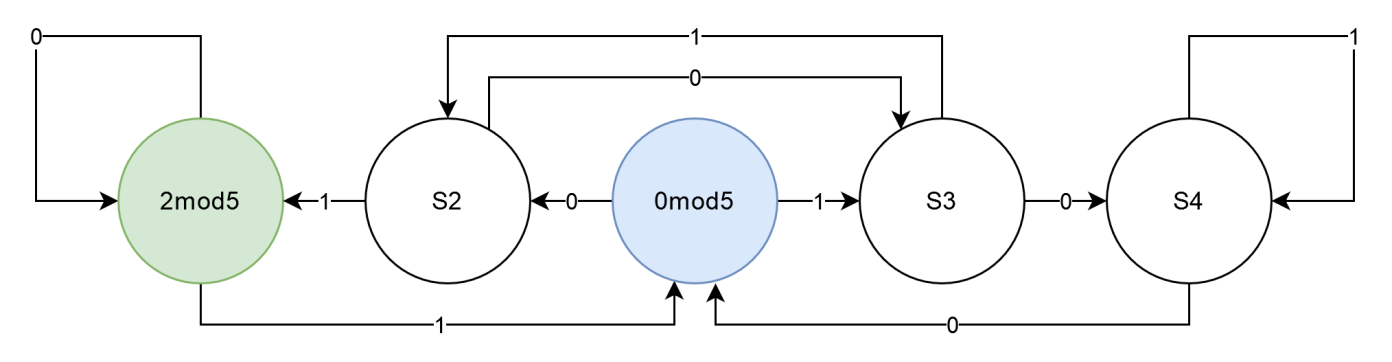
\includegraphics[scale = 0.3]{2c.png}
    \caption{solution 2.c}
    \label{fig.2c}
\end{figure}
\marginpar[]{\footnotesize{Bleu: État initial Vert: État acceptant}}
\end{document}